\begin{frame}{Bootstrap Regression Strategies}
    \begin{center}
    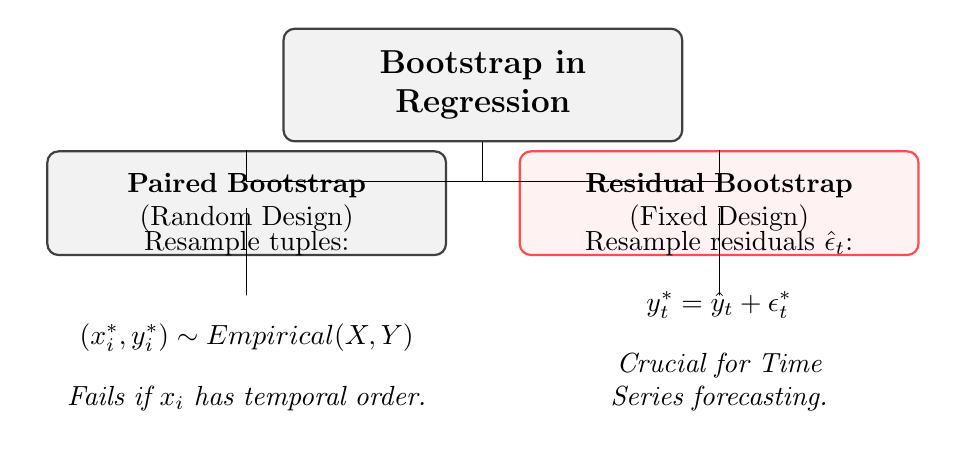
\begin{tikzpicture}[
        edge from parent path={(\tikzparentnode.south) -- ++(0,-0.5) -| (\tikzchildnode.north)},
        level 1/.style={sibling distance=6cm, level distance=1.5cm},
        box/.style={draw=darkgray, thick, rounded corners, fill=gray!10, text width=4.5cm, align=center, inner sep=8pt},
        highlight/.style={draw=red!70, fill=red!5, thick}
    ]

        \node[box, font=\bfseries\large] {Bootstrap in Regression}
            child {
                node[box] {\textbf{Paired Bootstrap}\\ (Random Design)}
                child {
                    node[box, draw=none, fill=none, text width=5cm] {
                        Resample tuples: \\
                        $$(x_i^*, y_i^*) \sim \text{Empirical}(X, Y)$$
                        \textit{Fails if $x_i$ has temporal order.}
                    }
                }
            }
            child {
                node[box, highlight] {\textbf{Residual Bootstrap}\\ (Fixed Design)}
                child {
                    node[box, draw=none, fill=none, text width=5cm] {
                        Resample residuals $\hat{\epsilon}_t$:
                        $$y_t^* = \hat{y}_t + \epsilon_t^*$$
                        \textit{Crucial for Time Series forecasting.}
                    }
                }
            };
    \end{tikzpicture}
    \end{center}
\end{frame}